\documentclass[11pt]{article}

\usepackage[margin=0.75cm]{geometry}
\usepackage{amsmath}
\usepackage{amssymb}
\usepackage{tikz}
\usepackage{enumitem}

\usetikzlibrary{arrows.meta}

\begin{document}

\twocolumn

\title{Problem Set 1, COSC330/PHYS306\\
Chapter 1 and Chapter 2-1 through 2-7}

\author{Prof. Jordan C. Hanson}

\maketitle

%===========================================================
% Chapter 1
%===========================================================

\section{Chapter 1}

\begin{enumerate}

%===========================================================
% Exercise 7
%===========================================================

\item For the pulse shown in Figure 1--60, graphically determine the following:

\begin{enumerate}[label=(\alph*)]
    \item rise time
    \item fall time
    \item pulse width
    \item amplitude
\end{enumerate}

\vspace{0.20cm}

\begin{center}
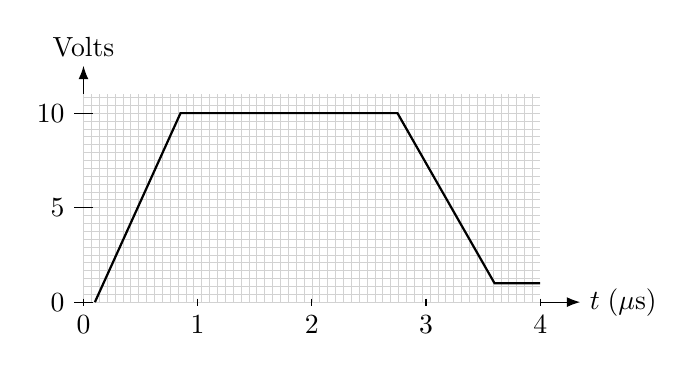
\begin{tikzpicture}[x=1.45cm,y=0.24cm,>=Latex]

% Axes
\draw[->] (0,0) -- (4.35,0)
    node[right] {$t\;(\mu\text{s})$};

\draw[->] (0,0) -- (0,12.5)
    node[above] {Volts};

% Grid
\draw[step=0.1cm,gray!35,very thin]
    (0,0) grid (4,11);

% Major x ticks
\foreach \x in {0,1,2,3,4}{
    \draw (\x,0.18) -- (\x,-0.18);
    \node[below] at (\x,-0.18) {\x};
}

% Major y ticks
\foreach \y/\lab in {0/0,5/5,10/10}{
    \draw (0.08,\y) -- (-0.08,\y);
    \node[left] at (-0.08,\y) {\lab};
}

% Pulse
\draw[thick]
    (0.10,0)
    -- (0.85,10)
    -- (2.75,10)
    -- (3.60,1)
    -- (4.00,1);

\end{tikzpicture}

\textbf{FIGURE 1--60}
\end{center}


%===========================================================
% Exercises 8--11
%===========================================================

\item Determine the period of the digital waveform in Figure 1--61.

\item What is the frequency of the waveform in Figure 1--61?

\item Is the pulse waveform in Figure 1--61 periodic or nonperiodic?

\item Determine the duty cycle of the waveform in Figure 1--61.

\vspace{0.20cm}

\begin{center}
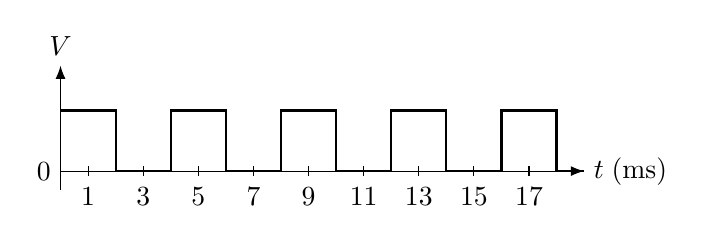
\begin{tikzpicture}[x=0.35cm,y=0.67cm,>=Latex]

% Axes
\draw[->] (0,0) -- (19,0)
    node[right] {$t\;(\text{ms})$};

\draw[->] (0,-0.35) -- (0,2.0)
    node[above] {$V$};

\node[left] at (0,0) {$0$};

% Tick marks
\foreach \x in {1,3,5,7,9,11,13,15,17}{
    \draw (\x,0.10) -- (\x,-0.10);
    \node[below] at (\x,-0.12) {\x};
}

% Waveform
\draw[thick]
    (0,1.15)
    -- (2,1.15)
    -- (2,0)
    -- (4,0)
    -- (4,1.15)
    -- (6,1.15)
    -- (6,0)
    -- (8,0)
    -- (8,1.15)
    -- (10,1.15)
    -- (10,0)
    -- (12,0)
    -- (12,1.15)
    -- (14,1.15)
    -- (14,0)
    -- (16,0)
    -- (16,1.15)
    -- (18,1.15)
    -- (18,0)
    -- (19,0);

\end{tikzpicture}

\vspace{0.10cm}

\textbf{FIGURE 1--61}
\end{center}


%===========================================================
% Exercises 12--14
%===========================================================

\item Determine the bit sequence represented by the waveform in Figure 1--62.
A bit time is $1\,\mu\text{s}$ in this case.

\item What is the total serial transfer time for the eight bits in Figure 1--62?
What is the total parallel transfer time?

\item What is the period if the clock frequency is $3.5\,\text{GHz}$?

\vspace{0.20cm}

\begin{center}
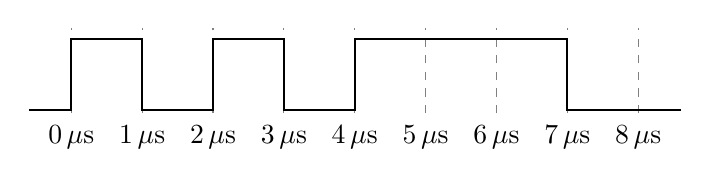
\begin{tikzpicture}[x=0.9cm,y=0.9cm,>=Latex]

% Bit boundary guide lines
\foreach \x in {0,1,2,3,4,5,6,7,8}{
    \draw[dashed,gray]
        (\x,-0.05) -- (\x,1.15);
}

% Waveform
\draw[thick]
    (-0.60,0)
    -- (0,0)
    -- (0,1)
    -- (1,1)
    -- (1,0)
    -- (2,0)
    -- (2,1)
    -- (3,1)
    -- (3,0)
    -- (4,0)
    -- (4,1)
    -- (7,1)
    -- (7,0)
    -- (8,0)
    -- (8.60,0);

% Time labels
\foreach \x in {0,1,2,3,4,5,6,7,8}{
    \node[below] at (\x,-0.08)
        {$\x\,\mu\text{s}$};
}

\end{tikzpicture}

\vspace{0.10cm}

\textbf{FIGURE 1--62}
\end{center}


%===========================================================
% Section 1-3
%===========================================================

\begin{center}
    {\large \textbf{Section 1--3 Basic Logic Functions}}
\end{center}


%===========================================================
% Exercises 15--18
%===========================================================

\item Form a single logical statement from the following information:

\begin{enumerate}[label=(\alph*)]
    \item The light is ON if SW1 is closed.
    \item The light is ON if SW2 is closed.
    \item The light is OFF if both SW1 and SW2 are open.
\end{enumerate}


\item A logic circuit requires HIGHs on all its inputs to make the output HIGH.
What type of logic circuit is it?


\item A basic 2-input logic circuit has a HIGH on one input and a LOW on the other
input, and the output is LOW. Identify the circuit.


\item A basic 2-input logic circuit has a HIGH on one input and a LOW on the other
input, and the output is HIGH. What type of logic circuit is it?

\end{enumerate}


%===========================================================
% Chapter 2
%===========================================================

\section{Chapter 2}

\begin{enumerate}

%===========================================================
% Chapter 2, Textbook Exercise 7
%===========================================================

\item Convert each binary number to decimal:

\begin{enumerate}[label=(\alph*)]
    \item $110011.11$
    \item $101010.01$
    \item $1000001.111$
    \item $1111000.101$
    \item $1011100.10101$
    \item $1110001.0001$
\end{enumerate}


%===========================================================
% Chapter 2, Textbook Exercise 8
%===========================================================

\item What is the highest decimal number that can be represented by each of the following numbers of binary digits (bits)?

\begin{enumerate}[label=(\alph*)]
    \item two
    \item three
    \item four
    \item five
    \item six
    \item seven
    \item eight
    \item nine
    \item ten
    \item eleven
\end{enumerate}


%===========================================================
% Chapter 2, Textbook Exercise 13
%===========================================================

\item Convert each number to binary using repeated division by 2:

\begin{enumerate}[label=(\alph*)]
    \item $15$
    \item $21$
    \item $28$
    \item $34$
    \item $40$
    \item $59$
    \item $65$
    \item $73$
\end{enumerate}


%===========================================================
% Chapter 2, Textbook Exercise 15
%===========================================================

\item Add the binary numbers:

\begin{enumerate}[label=(\alph*)]
    \item $11 + 01$
    \item $10 + 10$
    \item $101 + 11$
    \item $111 + 110$
    \item $1001 + 101$
    \item $1101 + 1011$
\end{enumerate}


%===========================================================
% Chapter 2, Textbook Exercise 25
%===========================================================

\item Express each decimal number as an 8-bit number in the 2's complement form:

\begin{enumerate}[label=(\alph*)]
    \item $+12$
    \item $-68$
    \item $+101$
    \item $-125$
\end{enumerate}


%===========================================================
% Chapter 2, Textbook Exercise 33
%===========================================================

\item Perform each addition in the 2's complement form:

\begin{enumerate}[label=(\alph*)]
    \item $10001100 + 00111001$
    \item $11011001 + 11100111$
\end{enumerate}

\end{enumerate}

\end{document}